\documentclass{article}

\usepackage[landscape]{geometry}
\usepackage{tikz}
\usepackage[utf8]{inputenc}

%\usetikzlibrary{shapes, geometric, arrows}

\tikzstyle{process} = [rectangle, minimum width = 2.5cm, minimum height = 1cm, 
	text centered, ultra thick, draw = black]
\tikzstyle{arrow} = [ultra thick, ->]

\begin{document}
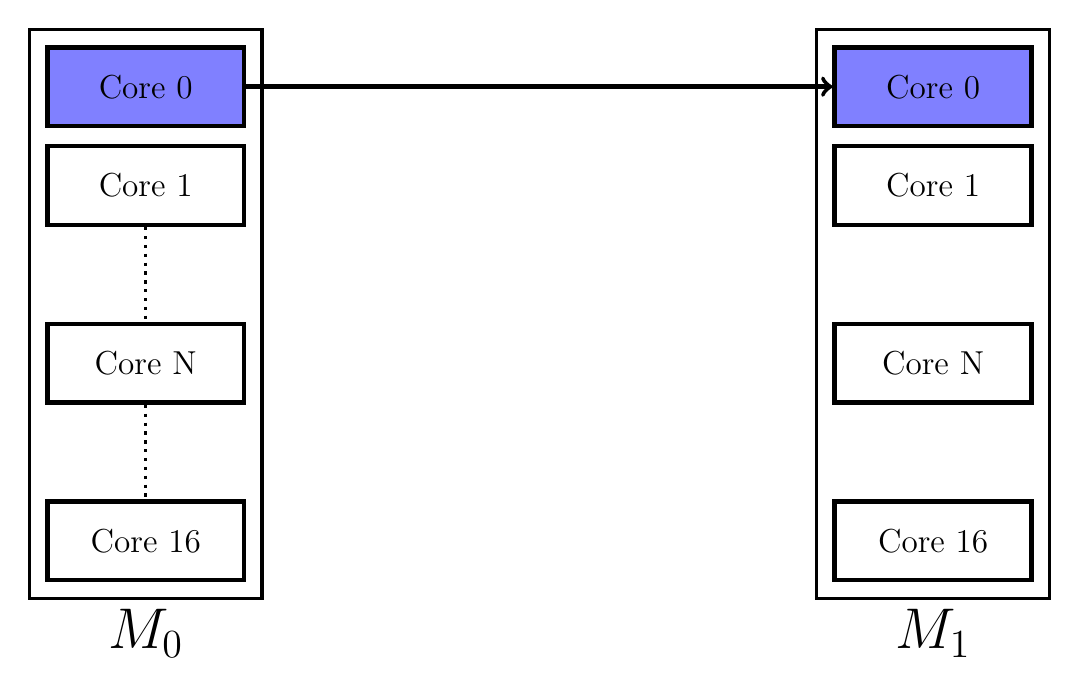
\begin{tikzpicture}[node distance = 10cm]

\node (M0) [matrix, draw = black, very thick, 
	inner sep = 2mm, row sep = 2mm, column sep = 2mm, 
	label = below:\huge $M_0$]
{
	\node (M00) [process, fill = blue!50] {\large Core 0}; \\

	\node (M01) [process] {\large Core 1}; \\[1cm]

	\node (M0N) [process] {\large Core N}; \\[1cm]

	\node (M016) [process] {\large Core 16}; \\
};

\draw [dotted, very thick] (M01) -- (M0N);
\draw [dotted, very thick] (M0N) -- (M016);

\node (M1) [matrix, draw = black, very thick, right of = M0, 
	inner sep = 2mm, row sep = 2mm, column sep = 2mm, 
	label = below:\huge $M_1$]
{
	\node (M10) [process, fill = blue!50] {\large Core 0}; \\

	\node (M11) [process] {\large Core 1}; \\[1cm]

	\node (M1N) [process] {\large Core N}; \\[1cm]

	\node (M116) [process] {\large Core 16}; \\
};

\draw [arrow] (M00) -- (M10);
\end{tikzpicture}
\end{document}
